\documentclass[a4paper,10pt]{article}
%\documentclass[a4paper,10pt]{scrartcl}

\usepackage[utf8]{inputenc}
\usepackage{hyperref}

\title{Floating Point Arithmetic Logic Unit}
\author{Suciu Andrei}
\date{October 2024}


\pdfinfo{%
  /Title    (Floating Point ALU)
  /Author   (Suciu Andrei)
  /Creator  ()
  /Producer ()
  /Subject  ()
  /Keywords ()
}



\usepackage{graphicx}
\usepackage{listings}
\usepackage{xcolor}
\graphicspath{ {images/} }

\definecolor{keywordsColor}{RGB}{101, 0, 153}
\lstset{
	language=VHDL,
	basicstyle=\ttfamily\footnotesize,
	keywordstyle=\color{keywordsColor}\bfseries,
	identifierstyle=\color{black},
	commentstyle=\color{gray},
	stringstyle=\color{green!60!black},
	numbers=left,
	numberstyle=\tiny\color{gray},
	stepnumber=1,
	tabsize=4,
	showstringspaces=false,
	breaklines=true,
	captionpos=b,
	frame=single,
	morekeywords={
		library, use, entity, architecture, signal, port, in, out, is, begin, end, std_logic, std_logic_vector,
		std_logic_1164, all, numeric_std, std_logic_arith, std_logic_unsigned, inout, to_integer, unsigned, signed,
		to_signed, to_unsigned
	}
}

\begin{document}
    \pagenumbering{gobble}
    \setlength{\parindent}{0pt}
    \begin{titlepage}
        \begin{center}
            \textbf{\large Department of Computer Science} \\[0.2cm]
            \textbf{\large Technical University of Cluj-Napoca} \\[0.5cm]
            
\includegraphics[width=1\textwidth]{utLogo.png} \\[1.0cm]

            \textbf{Floating Point Arithmetic Logic Unit} \\
            \textit{Laboratory activity 2024-2025} \\[4.0cm]

            Name: Suciu Andrei \\
            Group: 30431 \\
            Email: suciu.se.an@student.utcluj.ro\\

            \vfill

            Structure of Computer Systems\\[0.5cm]
            
\includegraphics[width=1\textwidth]{utLogo.png} \\[4.0cm]


        \end{center}
    \end{titlepage}
    \newpage

    \tableofcontents
    \newpage

    \pagenumbering{arabic}

    \section{Project Overview}
    \subsection{Specifications}
    Design an arithmetic logic unit on a 32-bit architecture capable of performing addition and multiplication operations on floating point numbers, encoded in the IEEE 754 standard. The ALU will be implemented on an FPGA, and must run and display various example operations.
    The ALU must be able to perform the following operations:
    \begin{itemize}
        \item 32-bit floating point addition
        \item 32-bit floating point multiplication
    \end{itemize}

    \subsection{Design}
    The implementation of the arithmetic logic unit will be designed in VHDL, using Vivado. The ALU will be contained within a master project which will provide the input and output display functionalities accoring to the FPGA provided at the laboratory. The project will be broken down into multiple smaller sources, each of which will be implemented using a behavioural style. Finally, all the project sources will be combined structurally to form a cohesive unit.

    \newpage

    \section{Bibliographic Research}
    \subsection{Arithmetic Logic Unit}
    In computing, an arithmetic logic unit (ALU) is a combinational digital circuit that is able to perform arithmetic on binary numbers. It is a fundamental building block of many other circuits, such as CPU or GPU.
    The ALU receives two input operands, an operation code, to decide which operation to perform, and optionally, a carry-in bit. Then, the result of the operation will be sent on the output signal.


    \subsection{Floating Point}
    In computing, numbers are represented in binary notation, as a series of bits, which can take values of either 1 or 0. In order to represent fractional parts, we must place a comma somewhere inside the number's representation. However, this greatly reduces the range of numbers which can be represented on a limitied amount of bits. In order to increase the range, we can imagine the comma moving (floating) left or right across the binary representation, according to what number we want to represent.

    Thus, we will to reserve a few bits for storing the position of the comma, creating a floating point number.

    \subsection{IEEE 754}
    The IEEE 754 defines the most widealy used standard for floating point numbers. Instead of storing the position of the comma, and the number itself, we will take advantage of scientific notation. In decimal scientific notation, the magnitude of the number is represented as a power of 10, and the "mantissa," essentially the core of the number, is stored as a fractional number between 1 and 10.

    Moving this format to binary, we can observe that no matter the number, the mantissa will always start with a leading "1." Thus, we can assume this part of the number and save 1 bit. The magnitude represents the exponent of a power of 2. Furthermore, there is one more bit for the sign of the number, 0 for positive, and 1 for negative.

    Overall, for a 32 bit number, the IEEE 754 standard formats the bits as such:
    \begin{itemize}
     \item 1 bit for the sign of the number
     \item 8 bits for the exponent
     \item 23 bits for the mantissa
    \end{itemize}

    The IEEE 754 standard also mentions the format for special values. There are five such numbers:
    \begin{itemize}
     \item Zero --- All exponent bits and all mantissa bits are set to $0$. Can be either positive or negative depending on the sign bit.
     \item Infinity --- All exponent bits are set to $1$, and all mantissa bits are set to $0$. Can be either positive or negative depending on the sign bit.
     \item NaN (Not a Number) --- All exponent bits are set to $1$, and at least one mantissa bit is set to $1$. The sign bit is not taken into consideration.
    \end{itemize}


    \section{Development Plan}
    \subsection{Development Overview}
    It is proposed that by each project meeting a different subsection of the Floating Point ALU will be completed, to be tested at the laboratory, and any irregularities in behaviour to be elliminated. By the end of the semester, the whole project must be completed and must be presented by the last week.

    \subsection{Project Lab 1}
    The project overview and development plan will be finalised and presented.

    \subsection{Project Lab 2}
    The supporting environment for the project must be implemented and tested on the FPGA. It must be capable of displaying numbers stored in a Read-Only Memory using a Seven-Segment Display, and must be capable of switching between multiple display modes using switches or buttons as input.

    \subsection{Project Lab 3}
    The floating point addition subsection of the ALU must be implemented as a separate circuit and must be fully functional.

    \subsection{Project Lab 4}
    The floating point mutliplication subsection of the ALU must be implemented as a separate circuit and must be fully functional.

    \subsection{Project Lab 5}
    Any remaining part of the project will be implemented, and the board's functionality will be fully tested. Any errors in the circuit's operations will be removed. The documentation will be updated as well, should the need arise.

    \newpage
    \section{Floating Point ALU Structure}
    The Operation of the Floating Point ALU is composed of three steps:
    \begin{enumerate}
     \item Check the validity of the inputs and the operation to be performed, and either proceed to the next step, or write the appropriate value and end the algorithm.
     \item Perform the operation, with all required steps.
     \item Realign the number to the IEEE 754 standard, and check for exponent overflow or underflow.
    \end{enumerate}

    In order to implement the Floating Point ALU, we will use Registers, Comparators, a smaller ALU capable of integer operations, a Wallace Tree Multiplier, and the Control Unit, implemented as a Finite State Machine.

    We can speed up the circuit by utilizing multiple comparators. For this implementation, we will use two comparators.

    \subsection{Algorithm}
    \subsubsection{Floating Point Adder}
    The Floating point Adder takes as inputs the two numbers, A and B, which are divided into their respective sign, exponent, and mantissa (with a 1 implicitly placed on the 24th bit.

    First, we compare the exponents, and the mantissa of the number with the smaller exponent is shifted to the right and its exponent is incremented until the exponents are equal. This way, the numbers are aligned to the same exponent.

    Next, we perform the addition of the mantissa. If the signs are equal, we simply add the two mantissas together, otherwise, we subtract the smaller mantissa from the larger one, and use the sign of the number with the larger mantissa for the result.

    Finally, we realign the resulting number to the IEEE-754 standard. If the mantissa has become too large, and there is a '1' on the 25th bit, we shift the result right and increment the exponent. If the mantissa is too small, we shift left and decrement the exponent until there is a '1' on exactly the 24th bit.

    \subsubsection{Floating Point Multiplier}
    The Floating Point Multiplier takes as inputs the two numbers, A and B, which are divided into their respective sign, exponent, and mantissa (with a 1 implicitly placed on the 24th bit.

    First, we add the two exponents together and subtract 127 from the resulting sum. This is because the exponents are implicitly stored as (127 + exponent).

    Next, we perform the multiplication on the mantissas. We can use a Wallace Tree Multiplier to perform the multiplication in a single clock cycle, which simplifies the circuit significantly.

    Since we use a standard 32 bit Wallace Tree Multiplier and the mantissa has only 24 bits, we extend with zero to the right. The two mantissas will always start with a 1 on the MSB, and by multiplying them, the resulting number will also have a 1 on the 64th bit. We simply select the next most significatn 23 bits for the result mantissa, with no need to shift and align the number.


    \subsection{Design}
    \subsubsection{ALU}
    \begin{figure}[h]
     \centering
     \caption{Simple Integer ALU}
     \includegraphics[scale=0.75]{adderALU.pdf}
    \end{figure}

    The ALU takes as input the two numbers, and a selection for which operation to be performed. Since it performs elementary operations, this is a combinational logic circuit, and requires no clock.\\
    The ouputs are the result of the operation, and an additional carry out bit, marked as \textit{cout}.\\
    The ALU is capable of performing four operations:
    \begin{itemize}
     \item Addition: \textit{result = numA + numB}
     \item Subtraction: \textit{result = numA - numB}
     \item Increment \textit{result = numA + 1}
     \item Decrement \textit{result = numA - 1}
    \end{itemize}
    In case of any overflow or underflow, the $cout$ bit is set to $1$, otherwise it remains $0$.

    \newpage
    \subsubsection{Comparator}
    The comparator takes as input two numbers, and the outputs $eq$ and $greater$ are set to $1$ if $numA > numB$ and if $numA = numB$ respectively.\\
    \begin{figure}[h]
     \centering
     \caption{Integer Comparator}
     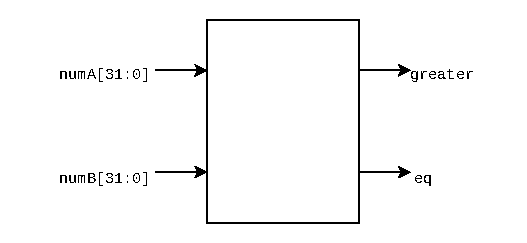
\includegraphics{comparator.pdf}
    \end{figure}


    \subsubsection{Multiplier}
    The mantissa multiplier was implemented as a wallace tree, capable of performing 32 bit multiplication. The result is on 64 bits. The desing was created recursively, starting from the 4 bit wallace tree multiplier. Each number is split into $Low$ and $High$, and then multiplied, shifted, and added accordingly.
    \begin{figure}[h]
     \centering
     \caption{Structure of Wallace Tree Multiplier}
     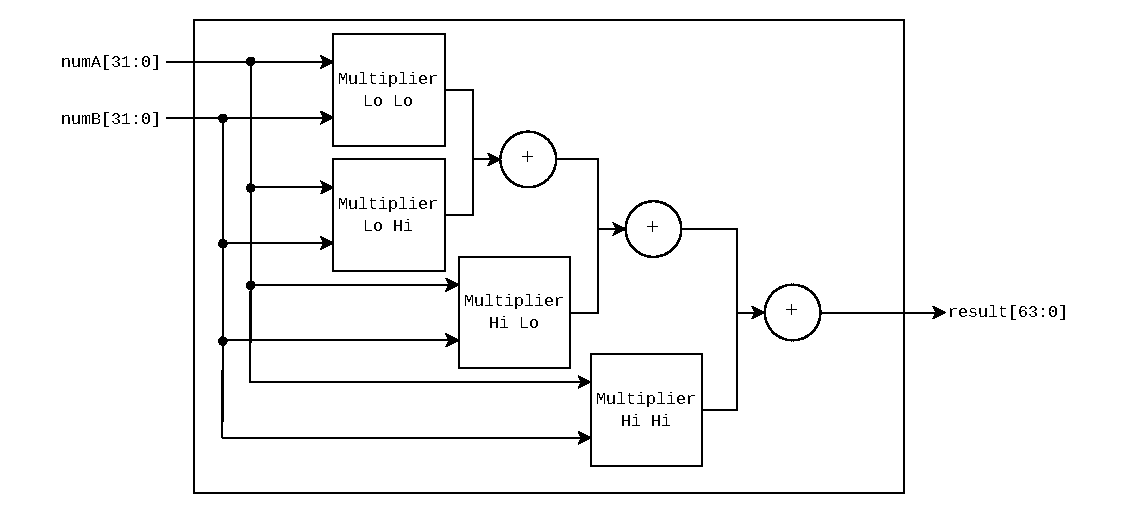
\includegraphics[scale=0.75]{multiplier.pdf}
    \end{figure}

    The entity for the Components used is available \hyperref[sec:components]{here}.

    \subsubsection{Control Unit}
    The Control Unit is the most complex part of the floating point adder. It is a finite state machine which controls all the select signals for the various components of the design. It switches states synchronously, and based on the state and results from differing components, sets the select signals for the multiplexers, the write signals for the registers, and the operation for the ALU.

    The Control Unit is a finite state machine with $22$ states, divided into $6$ groups:
    \begin{itemize}
      \item Idle: $idle\_state$\\
      Machine is idle and not busy performing any operation.
      \item Check Input: $check\_nan\_1,\ check\_nan\_2,\ check\_zero,\ valid\_op$\\
      Check the validity of the inputs and either proceed with the algorithm or write the result directly.
      \item Perform FP Addition: $fpAdd\_compare,\ fpAdd\_add$\\
      Shift mantissa and increment exponents until they are equal, then add the mantissas.
      \item Perform FP Multiplication: $fpMul\_add,\ fpMul\_sub127,\ fpMul_mul$\\
      Add the two exponents together, subtract $127$ from the result, and multiply the mantissas.
      \item Realign to Standard: $align,\ verify\_exponent\_overflow, verify\_exponent\_underflow$\\
      Realign mantissa to standard and check for overflow or underflow in the exponent.
      \item Write Special: $writeNan,\ writeInfinityXor,\ writeInfinityPos,\ writeInfinityNeg,\\ writeZeroXor,\ writeZeroPos,\ writeZeroNeg,\ writeNum1,\ writeNum2$\\
      Used when operation is invalid.
    \end{itemize}

    \begin{figure}[htbp]
    \centering
    \caption{The Control Unit transition diagram}
    \includegraphics[scale=0.7]{dot.pdf}
    \end{figure}

    The entity for the Control Unit is available \hyperref[sec:controlUnit]{here}.

    \newpage
    \subsubsection{Top Level Design}
    Following the design specifications, all the components were connected. A separate register was used for each part of the inputs and outputs, and two comparators were used to speed up the process. Multiplexers were used to switch between the inputs to the different components. Since there is more space in the register than is needed to store the mantissa, it is stored left aligned, and padded with $0$. Only the most significant bits from the mantissa register and multiplier result are used, ensuring there is never a mantissa overflow.

    \begin{figure}[htbp]
    \centering
    \caption{The top level design}
    \includegraphics[scale=0.5]{fpALU.pdf}
    \end{figure}


    \newpage
    \subsection{Implementation}
    The code for the Comparator, ALU, Control Unit and Registers was written in a behavioural stlye. The code for the Multiplier, and Top Level was written in a structural stlye.

    For ease of implementation, separate register components were written with a $4:1$, and an $8:1$ multiplexer included.\\
    The Top Level Design is mostly composed of port maps, with a couple of multiplexers for the ALU and Comparators.\\
    The Control Unit is a Finite State Machine composed of two processes:
    \begin{itemize}
     \item The first porcess calculates the next state of the machine. The switching between states is done synchronously. When checking the inputs, internal flags are set to $1$ or $0$, These flags and the operation input then form an address in a ROM which gives the next state.
     \item The second process represents a multitude of multiplexers and simple logic gates which caluclate the output signals based on the current state and the inputs given. This process is asynchronous.
    \end{itemize}

    The code for the ROM is available \hyperref[sec:ROM]{here}.


    \section{Testing}
    Testbenches were written for the Addition Operation and the Multiplication Operation. Multiple combinations of inputs were used, and the machines ability to detect wrong inputs was also tested.\\
    The inputs are captured immediately as the start value is read as $1$ on a rising edge of the clock. A change in inputs afterwards will not affect the performance.\\
    While the machine is busy, the working bit is set to $1$, otherwise, while it is idle it remains $0$. Once the algorithm is finished and the working bit is set to $0$, the output will remain stable. If the machine is started again, the output will still remain stable for at least $one$ clock cycle. Afterwards, it cannot be guaranteed what will appear on the output while the working flag is active.

    \subsection{Addition}
    \subsubsection{Regular Behaviour}
    The FP ALU performs as expected under regular circumstances. It is performs as expected when adding positive numbers, when adding negative numbers, and when adding zero to a number.\\
    \includegraphics[scale=0.5]{addRegular.png}

    \newpage
    \subsubsection{Special Cases}
    Based on the ROM in the Control Unit, the special cases for addition are as follows:
    \begin{itemize}
     \item $(+\infty) + (+\infty) = +\infty$
     \item $(+\infty) + (-\infty) = NaN$
     \item $(+\infty) + (\pm0) = +\infty$
     \item $(\pm \infty) + x = \pm \infty$
     \item $(-\infty) + (-\infty) = -\infty$
     \item $(-\infty) + (\pm0) = -\infty$
     \item $(\pm0) + (\pm0) = +0$
     \item $(\pm0) + (\mp0) = +0$
     \item $(\pm0) + x = +0$
    \end{itemize}
    Also including their reciprocals.
    These special cases were tested, and the correct result was given.\\
    \includegraphics[scale=0.5]{addSpecial.png}

    The code for the Add Testebench is available \hyperref[sec:AddTest]{here}.

    \subsection{Multiplication}
    \subsubsection{Regular Beheviour}
    Under regular circumstances the multiplication is performed correctly. When multiplying numbers with the same sign, the resulting sign is positive, and when multiplying with 0, the result will also be 0, with the same logic applied for the sign.\\
    \includegraphics[scale=0.5]{mulRegular.png}

    \newpage
    \subsubsection{Special Cases}
    Based on the ROM in the Control Unit, the special cases for addition are as follows:
    \begin{itemize}
     \item $(\pm\infty) * (\pm\infty) = +\infty$
     \item $(\pm\infty) * (\mp\infty) = -\infty$
     \item $(\pm\infty) * (\pm0) = NaN$
     \item $(\pm\infty) * (\mp0) = NaN$
     \item $(\pm\infty) * x = (XOR)\infty$
     \item $(-\infty) + (\pm0) = -\infty$
     \item $(\pm0) * (\pm0) = +0$
     \item $(\pm0) * (\mp0) = -0$
     \item $(\pm0) * x = (XOR)0$
    \end{itemize}
    Also including their reciprocals.
    These special cases were tested, and the correct result was given.\\
    \includegraphics[scale=0.5]{mulSpecial.png}

    The code for the Mul Testebench is available \hyperref[sec:MulTest]{here}.
    \newpage
    \section{Code}
    \label{sec:components}
    \subsection{ALU}
    \begin{lstlisting}
    entity alu32bit is
    Port (
            numA : in STD_LOGIC_VECTOR (31 downto 0);
            numB : in STD_LOGIC_VECTOR (31 downto 0);
            op : in STD_LOGIC_vector(1 downto 0);
            output : out STD_LOGIC_VECTOR (31 downto 0);
            cout: out std_logic);
    end alu32bit;
    \end{lstlisting}

    \subsection{Comparator}
    \begin{lstlisting}
    entity comparator32bit is
    Port ( numA : in STD_LOGIC_vector(31 downto 0);
           numB : in STD_LOGIC_vector(31 downto 0);
           eq : out STD_LOGIC;
           greater : out STD_LOGIC);
    end comparator32bit;
    \end{lstlisting}

    \subsection{Register with multiplexer}
    \begin{lstlisting}
     entity register32bitW4x1Mux is
    Port ( A : in STD_LOGIC_VECTOR (31 downto 0);
           B : in STD_LOGIC_VECTOR (31 downto 0);
           C : in STD_LOGIC_VECTOR (31 downto 0);
           D : in STD_LOGIC_VECTOR (31 downto 0);
           S: in std_logic_vector(1 downto 0);
           write : in STD_LOGIC;
           clk : in STD_LOGIC;
           output : out STD_LOGIC_VECTOR (31 downto 0));
    end register32bitW4x1Mux;
    \end{lstlisting}

    \subsection{Wallace Tree Multiplier}
    \begin{lstlisting}
    entity multiplier32bit is
    Port ( numA : in STD_LOGIC_VECTOR (31 downto 0);
           numB : in STD_LOGIC_VECTOR (31 downto 0);
           result : out STD_LOGIC_VECTOR (63 downto 0));
    end multiplier32bit;
    \end{lstlisting}

    \newpage
    \label{sec:controlUnit}
    \subsection{Control Unit}
    \begin{lstlisting}
    entity controlUnit is
    Port (
      clk : in STD_LOGIC;
      reset: in std_logic;
      start:in std_logic;
      op:in std_logic;

      writeSign1:out std_logic;
      writeSign2:out std_logic;
      writeSignRes:out std_logic;

      writeExponent1:out std_logic;
      writeExponent2:out std_logic;
      writeExponentRes:out std_logic;

      writeMantissa1:out std_logic;
      writeMantissa2:out std_logic;
      writeMantissaRes:out std_logic;

      selectSign1:out std_logic_vector(1 downto 0);
      selectExponent1:out std_logic_vector(1 downto 0);
      selectMantissa1:out std_logic_vector(1 downto 0);

      selectSign2:out std_logic_vector(1 downto 0);
      selectExponent2:out std_logic_vector(1 downto 0);
      selectMantissa2:out std_logic_vector(1 downto 0);

      selectSignRes:out std_logic_vector(2 downto 0);
      selectExponentRes:out std_logic_vector(2 downto 0);
      selectMantissaRes:out std_logic_vector(2 downto 0);

      outSign1:in std_logic;
      outSign2:in std_logic;
      outSignRes:in std_logic;
      outMantissaRes31:in std_logic;

      comparator1Select:out std_logic_vector(2 downto 0);
      comparator1Eq:in std_logic;
      comparator1Greater:in std_logic;

      comparator2Select:out std_logic_vector(2 downto 0);
      comparator2Eq:in std_logic;
      comparator2Greater:in std_logic;

      alu32bitOp:out std_logic_vector(1 downto 0);
      alu32bitSelect:out std_logic_vector(2 downto 0);
      alu32bitCout: in std_logic;

      infinityFlag:out std_logic;
      zeroFlag:out std_logic;
      nanFlag:out std_logic;

      working:out std_logic
    );
    end controlUnit;
    \end{lstlisting}

    \newpage
    \label{sec:aluTop}
    \subsection{ALU Top level}
    \begin{lstlisting}
    entity aluFloat is
    Port (
        clk : in STD_LOGIC;
        start:in std_logic;
        reset:in std_logic;
        op : in STD_LOGIC;

        num1 : in STD_LOGIC_VECTOR (31 downto 0);
        num2 : in STD_LOGIC_VECTOR (31 downto 0);

        res : out STD_LOGIC_VECTOR (31 downto 0);
        working:out std_logic;
        infinityFlag:out std_logic;
        zeroFlag:out std_logic;
        nanFlag:out std_logic
    );
    end aluFloat;
    \end{lstlisting}

    \label{sec:ROM}
    \subsection{ROM}
    \begin{lstlisting}
    case internalFlags is
--		internalFlags<=op & infinityPos1 & infinityNeg1 & infinityPos2 & infinityNeg2 &
--				zeroPos1 & zeroNeg1 & zeroPos2 & zeroNeg2;
			when "000000000"=>
				state<=fpAdd_compare;

			-- +infinity + x
			when b"0_10_10_00_00"=> -- +inf + +inf
				state<=writeInfinityPos;
			when b"0_10_01_00_00"=> -- +inf + -inf
				state<=writeNan;
			when b"0_10_00_00_10"=> -- +inf + +0
				state<=writeInfinityPos;
			when b"0_10_00_00_01"=> -- +inf + -0
				state<=writeInfinityPos;
			when b"0_10_00_00_00"=> -- +inf + x
				state<=writeInfinityPos;

			-- -infinity + x
			when b"0_01_10_00_00"=> -- -inf + +inf
				state<=writeNan;
			when b"0_01_01_00_00"=> -- -inf + -inf
				state<=writeInfinityNeg;
			when b"0_01_00_00_10"=> -- -inf + +0
				state<=writeInfinityNeg;
			when b"0_01_00_00_01"=> -- -inf + -0
				state<=writeInfinityNeg;
			when b"0_01_00_00_00"=> -- -inf + x
				state<=writeInfinityNeg;

			-- +0 + x
			when b"0_00_10_10_00"=> -- +0 + +inf
				state<=writeInfinityPos;
			when b"0_00_01_10_00"=> -- +0 + -inf
				state<=writeInfinityNeg;
			when b"0_00_00_10_10"=> -- +0 + +0
				state<=writeZeroPos;
			when b"0_00_00_10_01"=> -- +0 + -0
				state<=writeZeroPos;
			when b"0_00_00_10_00"=> -- +0 + x
				state<=writeNum2;

			-- -0 + x
			when b"0_00_10_01_00"=> -- -0 + +inf
				state<=writeInfinityPos;
			when b"0_00_01_01_00"=> -- -0 + -inf
				state<=writeInfinityNeg;
			when b"0_00_00_01_10"=> -- -0 + +0
				state<=writeZeroPos;
			when b"0_00_00_01_01"=> -- -0 + -0
				state<=writeZeroNeg;
			when b"0_00_00_01_00"=> -- -0 + x
				state<=writeNum2;

			-- x + special
			when b"0_00_10_00_00"=> -- x + +inf
				state<=writeInfinityPos;
			when b"0_00_01_00_00"=> -- x + -inf
				state<=writeInfinityNeg;
			when b"0_00_00_00_10"=> -- x + +0
				state<=writeNum1;
			when b"0_00_00_00_01"=> -- x + -0
				state<=writeNum1;

--		internalFlags<=op & infinityPos1 & infinityNeg1 & infinityPos2 & infinityNeg2 &
--				zeroPos1 & zeroNeg1 & zeroPos2 & zeroNeg2;
			when "100000000"=>
				state<=fpMul_add;

			-- +infinity * x
			when b"1_10_10_00_00"=> -- +inf * +inf
				state<=writeInfinityPos;
			when b"1_10_01_00_00"=> -- +inf * -inf
				state<=writeInfinityNeg;
			when b"1_10_00_00_10"=> -- +inf * +0
				state<=writeNan;
			when b"1_10_00_00_01"=> -- +inf * -0
				state<=writeNan;
			when b"1_10_00_00_00"=> -- +inf * x
				state<=writeInfinityXor;

			-- -infinity * x
			when b"1_01_10_00_00"=> -- -inf * +inf
				state<=writeInfinityNeg;
			when b"1_01_01_00_00"=> -- -inf * -inf
				state<=writeInfinityPos;
			when b"1_01_00_00_10"=> -- -inf * +0
				state<=writeNan;
			when b"1_01_00_00_01"=> -- -inf * -0
				state<=writeNan;
			when b"1_01_00_00_00"=> -- -inf * x
				state<=writeInfinityXor;

			-- +0 * x
			when b"1_00_10_10_00"=> -- +0 * +inf
				state<=writeNan;
			when b"1_00_01_10_00"=> -- +0 * -inf
				state<=writeNan;
			when b"1_00_00_10_10"=> -- +0 * +0
				state<=writeZeroPos;
			when b"1_00_00_10_01"=> -- +0 * -0
				state<=writeZeroNeg;
			when b"1_00_00_10_00"=> -- +0 * x
				state<=writeZeroXor;

			-- -0 * x
			when b"1_00_10_01_00"=> -- -0 * +inf
				state<=writeNan;
			when b"1_00_01_01_00"=> -- -0 * -inf
				state<=writeNan;
			when b"1_00_00_01_10"=> -- -0 * +0
				state<=writeZeroNeg;
			when b"1_00_00_01_01"=> -- -0 * -0
				state<=writeZeroPos;
			when b"1_00_00_01_00"=> -- -0 * x
				state<=writeZeroXor;

			-- x * special
			when b"1_00_10_00_00"=> -- x * +inf
				state<=writeInfinityXor;
			when b"1_00_01_00_00"=> -- x * -inf
				state<=writeInfinityXor;
			when b"1_00_00_00_10"=> -- x * +0
				state<=writeZeroXor;
			when b"1_00_00_00_01"=> -- x * -0
				state<=writeZeroXor;

			when others=>
				state<=writeNan;
		end case;
    \end{lstlisting}

    \newpage
    \subsection{Testbenches}
    \label{sec:AddTest}
    \lstinputlisting[caption=Add Testbench]{code/AddTB.txt}

    \newpage
    \label{sec:MulTest}
    \lstinputlisting[caption=Mul Testbench]{code/MulTB.txt}

    \newpage
    \section{Bibliography}
    \begin{thebibliography}{9}
      \bibitem{Steven Petryk}
        Steven Petryk,
        \href{https://www.youtube.com/watch?v=mKJiD2ZAlwM}{Adding IEEE-754 Floating Point Numbers},
        Oct 2015

      \bibitem{wikipediaFloat}
        Wikipedia,
        \href{https://en.wikipedia.org/wiki/IEEE_754}{IEEE 754},
        Oct 2024

      \bibitem{jan Misali}
        Jan Misali,
        \href{https://www.youtube.com/watch?v=dQhj5RGtag0}{how floating point works},
        May 2022
    \end{thebibliography}



\end{document}
